\documentclass[conference]{IEEEtran}
\IEEEoverridecommandlockouts


\usepackage[backend=biber]{biblatex}
\usepackage{amsmath,amssymb,amsfonts}
\usepackage{algorithmic}
\usepackage{graphicx}
\usepackage{textcomp}
\usepackage{xcolor}
\def\BibTeX{{\rm B\kern-.05em{\sc i\kern-.025em b}\kern-.08em
    T\kern-.1667em\lower.7ex\hbox{E}\kern-.125emX}}
\bibliography{amci_references}
\begin{document}

\title{Mobile Augmented Reality\\
}

\author{\IEEEauthorblockN{1\textsuperscript{st} Matthias Kerat 2\textsuperscript{nd} Mario Schlagenweith 3\textsuperscript{st} Marcel Kohnle}
\IEEEauthorblockA{\textit{Fortgeschrittene Mensch Computer Interaktion, Masterstudiengang Hochschule Aalen}\\
Aalen, Deutschland\\
matthias.kerat@studmail.htw-aalen.de, mario.schlagenweith@studmail.htw-aalen.de, marcel.kohnle@studmail.htw-aalen.de}
}

\maketitle

\begin{abstract}
This document is a model and instructions for \LaTeX.
This and the IEEEtran.cls file define the components of your paper [title, text, heads, etc.]. *CRITICAL: Do Not Use Symbols, Special Characters, Footnotes, 
or Math in Paper Title or Abstract.
\end{abstract}

\begin{IEEEkeywords}
component, formatting, style, styling, insert
\end{IEEEkeywords}

\section{Introduction}
This document is a model and instructions for \LaTeX.
Please observe the conference page limits. 



\section{Kernprinzipien und zentrale Begriffe}

Bei AR-Systemen wird zuerst die reale Welt, die hierbei das Ziel darstellt, erkannt und festgehalten. Dazu gehören beispielsweise meschliche Körper, Räume oder freie Flächen. Nach der Erkennung wird die virtuelle Welt dem Erweiterungszweck nach modelliert. Anschließend werden die digitalen Informationen auf die reale Welt projiziert, um diese zu erweitern. Dieses Konzept lässt sich in drei zentrale Schritte unterteilen: Erkennen, Festhalten und Zusammenführen. In den folgenden Sektionen werden vier verschiedene AR-Grundprinzipien aufgeführt, die sich teilweise überschneiden, jedoch als wichtige Begrifflichkeiten gelten.\autocite{amin2015comparative}

\subsection{Markerbasiertes Konzept}
Das markerbasierte Konzept wird auch als Bilderkennung bezeichnet. Dabei werden eine Kamera und ein sichtbarer Marker wie beispielsweise ein QR-Code verwendet. Applikationen, die nach diesem Konzept vorgehen, können über die Kamera den Marker von anderen Gegenständen unterscheiden. Der Markererkennungsalgorithmus geht dabei wie folgt vor:
\begin{enumerate}
	\item Aufgenommene Bilder in verschiedene Regionen unterteilen
	\item Bilder in den verschiedenen Regionen erkennen
	\item Regionen in Segmente aufteilen
	\item Segmente durch Linien trennen
	\item Linien über die Segmentgrenzen hinaus erweitern
	\item Linien mit Ecken festhalten
	\item Marker finden
\end{enumerate}
\autocite{aggarwal2019augmented} Die zuverlässige Erkennung des Markers hängt stark von dessen Eigenschaften ab. Zum Beispiel sind Unterschiede in der Helligkeit im Gegensatz zur Auseinanderhaltung verschiedener Farben einfacher, was an dem schlechten automatischen Weißabgleich der Kameras liegt. Deshalb sind schwarz-weise Marker optimal. Ein markerbasiertes System sollte zudem in der Lage sein, die Lage der Kamera anhand des erkannten Markers zu berechnen. Dabei reichen vier bekannte Punkte aus, um die Lage zuverlässig zu bestimmen. Viele Systeme verwenden daher schwarz-weise, quadratische Marker.\autocite{siltanen2012theory} Ein anderer Ansatz einer markerbasierten Erkennung ist der Einsatz eines aktiven Markers, der ein Signal, wie beispielsweise ein Licht oder ein magnetisches Feld, aussendet, das wahrgenommen werden kann.\autocite{bostanci2013user}

\subsection{Markerloses Konzept}
Dieses Konzept ist auch bekannt als ortsbasierte Realität und benötigt beim Festlegen der virtuellen Erweiterungen keinen extra für die Erkennung platzierten physikalischen Marker. Die zum Bestimmen des Orts erforderlichen Daten können dabei von digitalen Kompassen, Geschwindigkeitssensoren oder GPS kommen. Diese sind beispielsweise in modernen Smartphones ab Werk enthalten und können für das markerlose Konzept durch eine entsprechende Schnittstelle verwendet werden. Anders als beim markerbasierten Konzept beschränkt sich die Aufgabe des Algorithmus hier auf die Identifikation verschiedener Muster und Farben anhand der empfangenen Daten.\autocite{aggarwal2019augmented} Die Erkennungs-und Registrierungstechniken sind jedoch meist komplizierter in markerlosen AR-Applikationen. Grundsätzlich fallen alle Gegenstände, die in der realen Welt vorkommen und nicht speziell für die Erkennung positioniert wurden, jedoch für AR-Tracking eingesetzt werden, in die Definition des markerlosen Konzepts. Das markerlose Konzept kann weiter unterteilt werden in modellbasierte Erkennung und Bewegungserkennung. Bei ersterem ist bereits vor dem Start der Erkennung Wissen über die reale Welt vorhanden und in einem dreidimensionalen Modell gespeichert. Letzteres hingegen basiert auf Abschätzungen ohne vorheriges Wissen der aktuellen Szene, die während des Trackings erfasst wird.\autocite[S. 39]{lima2009model}

\subsection{Verfolgung natürlicher Merkmale}
Beim Verfolgen natürlicher Merkmale werden keine speziell generierten Marker benötigt, sondern es geht um eine bildverarbeitungsbasierte Erkennungstechnik, die Objekte erfasst, die sich im natürlichen Umfeld eines aufgenommenen Bildes befinden. Darunter fallen beispielsweise Ecken, Kanten oder Tröpfchen. Abbildung \ref{fig:1} zeigt den vereinfachten Ablauf einer Erkennungspipeline, um Schlüsselpunkte eines Objekts zu bestimmen.
\begin{figure}[htbp]
	\centering
	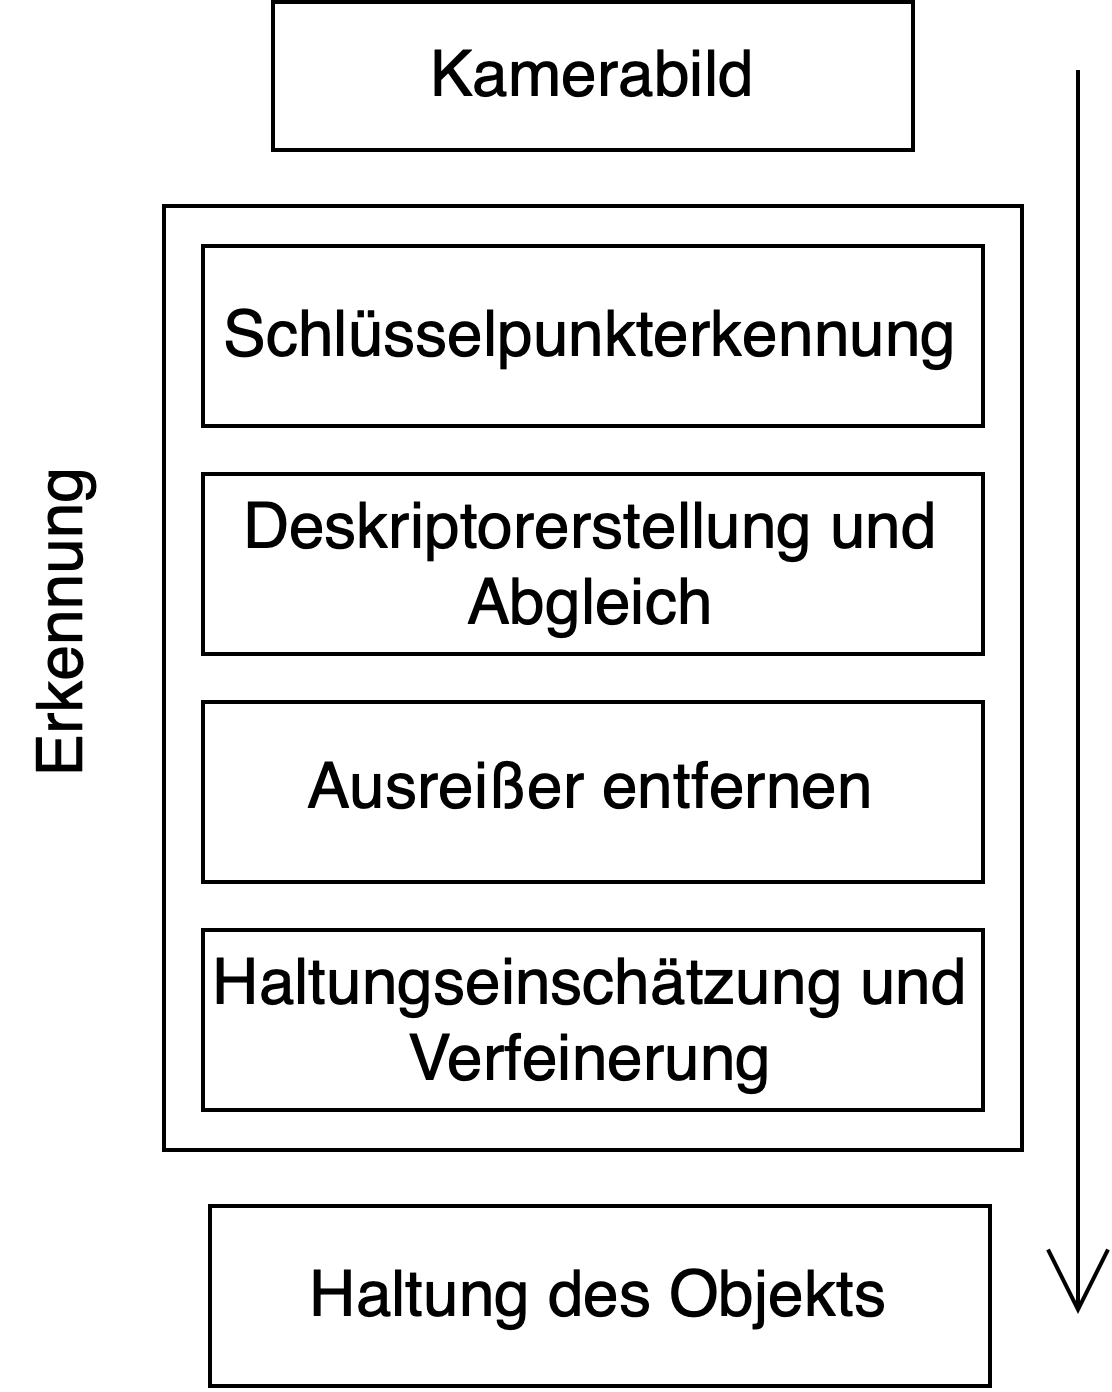
\includegraphics[width=0.25\textwidth]{images/natural_feature_tracking.png}
	\caption{Erkennungspipeline - Darstellung nach \autocite[S. 28]{cukovic2015marker}}
	\label{fig:1}
\end{figure}
Bei Phase zwei stehen unterschiedliche Deskriptoren zur Verfügung. Bei der skalierungsinvariaten Merkmalstransformation werden beispielsweise dominierende Schlüsselpunktausrichtungen unter Verwendung von Gradienten berechnet. In einem weiteren Schritt werden alle Deskriptoren und deren Position im Originalbild in einer Datenbank gespeichert. Anschließend vergleicht der Algorithmus in Echtzeit neue Deskriptoren mit den bereits abgespeicherten. In der nächsten Phase werden Außreiser mit Hilfe von aufsteigend aufwendigen Schlüsselpunktentfernungstechniken herausgelöst bevor dann die Ausrichtung geschätzt wird. Als letzter Schritt erfolgt basierend auf der Gauss-Newton-Iteration eine Verfeinerung des Ergebnisses, um Reprojektionsfehler der Schlüsselwerte zu minimieren.\autocite[S. 28 f.]{cukovic2015marker}





\renewcommand*{\bibfont}{\small}
\printbibliography
\end{document}
